\documentclass{article}

\title{ \textbf{ Design \& Analysis of Algorithms} \\
Kruskal’s algorithm Investigation }
\author{Axel Solano}
\usepackage{geometry}
 \geometry{
 a4paper,
 total={170mm,257mm},
 left=30mm,
    right=30mm,
 top=25mm,
 }
\usepackage{amsmath}
\usepackage{mathtools}
\DeclarePairedDelimiter\ceil{\lceil}{\rceil}
\usepackage{listings}
\usepackage{graphicx}
\usepackage[export]{adjustbox}
\usepackage{float}
\usepackage[dvipsnames]{xcolor}
\lstloadlanguages{Ruby}
\lstset{%
basicstyle=\ttfamily,
commentstyle = \ttfamily\color{green},
keywordstyle=\ttfamily\color{red},
stringstyle=\color{blue}}
\lstset{
numbers=left,
numberstyle=\small,
numbersep=8pt,
language=Ruby}

\begin{document}
\pagenumbering{gobble}
\maketitle
\pagenumbering{arabic}
\tableofcontents
\newpage

\section{Introduction}
In this program, I am going to use the scientific method to demonstrate that Kruskal’s algorithm runs in O(m log(n)) time, in which m in the the number of edges  and n is the number of vertices in an undirected graph.

\section{Analysis of Kruskal’s algorithm}
The algorithm is going to be divide in three parts. The first part is the construction of the heap with the list of edges. The second part is the construction of a Hash that will contain the id of the vertex as an identifier and each of them will contain a cluster of the respective vertex. The last part consists of building the spanning tree.\\


\begin{lstlisting}[language=ruby]
def mstKruskal(graph)
    tree = []
    # List of edges to return as spanning tree

    @h = MinHeap.new
    # Priority Queque that will use the weight of
    #edges as key

    mapp = Hash.new
    #Hash that will save the cluster for every vertices

    cluster = Cluster.new
    #Cluster is a data structure for the creation,
    #find and union of clusters in vertices


    #The first part is creating the heap
    lista = graph.list_edges
    @h.buildHeap(lista)


    #The second part is saving every cluster for
    #each vertex in the Hash
    listvertices = graph.list_vertices
    listvertices.each do |v|
      mapp[v.getId] = cluster.makeSet(v)
    end

    #The third part is to return the spanning tree
    i = 1
    n = @h.getSize
    while ( tree.length!=lista.length-1 &&  i<=n )
      i = i + 1
      edge = @h.removeMin(lista)
      v1 = edge.getEndVertices.fetch(0)
      v2 = edge.getEndVertices.fetch(1)
      a = cluster.findParent(mapp[v1.getId])
      b = cluster.findParent(mapp[v2.getId])
      if a != b
        tree.push(edge)
        cluster.union(a,b)
      end
    end

    return tree
  end
\end{lstlisting}

\subsection{Theorethical Analysis}
\subsubsection{Heap}
In this part, I used the same implementation from the last assigment but I modify from a max-Heap to min-Heap. The function buildHeap() which construct the heap maintain the same time complexity as O(n) and the function removeMin() also maintain the time complexity of O(log(n)).\\

\paragraph{buildHeap:}This function check from the bottom of the tree to the top and the number of operations in each node is equivalent to the distance between the current level of the tree and the last level. The last level of the tree is founded on the nodes after the division by two of the total number nodes of the tree. In this theoretical analysis, I assume that the operations of each node are in the worst case scenario.

$$\sum_{i=1}^{h} 2^{h-i} i$$\\
\\
Reducing the expression

$$\sum_{i=1}^{h} 2^{h-i} i = 2^{h} \sum_{i=1}^{h} \frac{i}{2^{i}} $$

$$\sum_{i=1}^{h} \frac{i}{2^{i}}  = 1 + \sum_{j=1}^{h-1} \frac{1}{2^{j}}  - \frac{h}{2^{h+1}}$$

$$1 + \sum_{j=1}^{h-1} \frac{1}{2^{j}}  - 2^{\frac{h}{2^{h+1}}} = 1 + 1 - \frac{1}{2^{h-1}}  - \frac{h}{2^{h+1}}$$

$$ 2^{h} \sum_{i=1}^{h} \frac{i}{2^{i}} = 2^{h} [2 - \frac{1}{2^{h-1}}  - \frac{h}{2^{h+1}} ]$$

$$\sum_{i=1}^{h} 2^{h-i} i =  2^{h} \sum_{i=1}^{h} \frac{i}{2^{i}} = 2^{h+1} - 2 - \frac{h}{2} $$\\

Then, make the h = log(n/2) where n is equal to the number of nodes. Therefore, the build function has the equation of:

$$T(n) = n - \frac{log(n)}{2} - 3 $$\\

This equation can be reduced in Big-Oh notation as O(m) in which m is the number of edges.\\\\

\paragraph{removeMin:}This function removes the minimum element in O(1) and then re-arrange the heap for next removal. The re-arragement time takes O(log(n)) because in each iteration the modification and those operations are equivalent to the level of the tree. Also, it is possible to find a relation between the level and the number of nodes of the tree.

$$ 1+2+4+···+ 2^{h-1}= 2^{h} −1 $$

$$ n <= 2^{h} −1 $$
$$ n + 1 <= 2^{h}  $$\\

Then, I take logarithms of both sides of these two inequalities\\

$$ log(n + 1) <= h $$

Finally, we can generalize\\

$$ h = \ceil{log(n + 1)} $$

$$T(n) = log(n + 1) = log(n) $$\\

This equation can be reduced in Big-Oh notation as O(log(m)) in which m is the number of edges.\\\\

\subsubsection{Hash}
In this part, the theoretical analysis is beyond the scope of the course but based on the book, this data structure present search function in time complexity O(1) in average case and in worst case scenario is in O(n) in which n is the lenght of the hash. In addtion, I will evaluate the time complexity of the search function empirically in the next section to proof that it doesn't have much influence in the performance of the kruskal's algorithm.Also, implementing the cluster with th map will cause a time complexity of O(n) in which n is the number of vertices.\\\\

\subsubsection{Return of the Spanning Tree}
In this part, there is a relevant implementation which is the Cluster class. This class use a Set class in which store the store the element and has linked-connection to itself with the name of parent. The purpose of these classes is to create the cluster of the spanning tree at the same time is creating the spanning tree. On the book, there is an implementaion called for Union-Find Structures called Tree-based implementation in which the idea behind is to perform search and insertion in O(log(n)) but with a path compression, this implementation can become faster but it's difficult to measure. The function is represented as $\alpha$(n) which less than or equal to log(n) and is called the Ackermann function.\\
In addition, the time complexity of the loop is represented as O(mlog(m)) in which m is the number of edges. However, we can change the m inside the logarithm function as function of n which is the number of vertices. The total number of edges possible in graph based on number of vertices is:\\

$$  \frac{n*(n-1)}{2} + n = m$$\\
The first part which is $\frac{n*(n-1)}{2} $ represent the total number of distinct edges that can be formed and the $n$ represent the loops edges of each vertex. Therefore, I am going to show the steps to obtain O(mlog(n)).

$$ T(n) = m*log(\frac{n*(n-1)}{2} + n)$$
Elimate the $n$ becuase loops edges is not allowed to create spannig trees.
$$ T(n) = m*log(\frac{n*(n-1)}{2})$$
$$ T(n) = m*log(\frac{n*(n-1)}{2})$$
$$ T(n) = m*log(n*(n-1)) - m*log(2)$$
$$ T(n) = m*log(n) + m*log(n-1) - m$$\\

This equation can be reduced in Big-Oh notation as O(mlog(n)).\\

Finally, the summation of the previous time complexities in Big-Oh notation of the used functions is O(m) + O(n) + O(mlog(n)) = O(mlog(n)).


\subsection{Empirical Analysis}


\subsubsection{Hash}
Based on the empirical analysis, the hash follow a constant uniform distribution which makes our assumption of constant time complexity correctly.
\begin{figure}[H]
\centering
  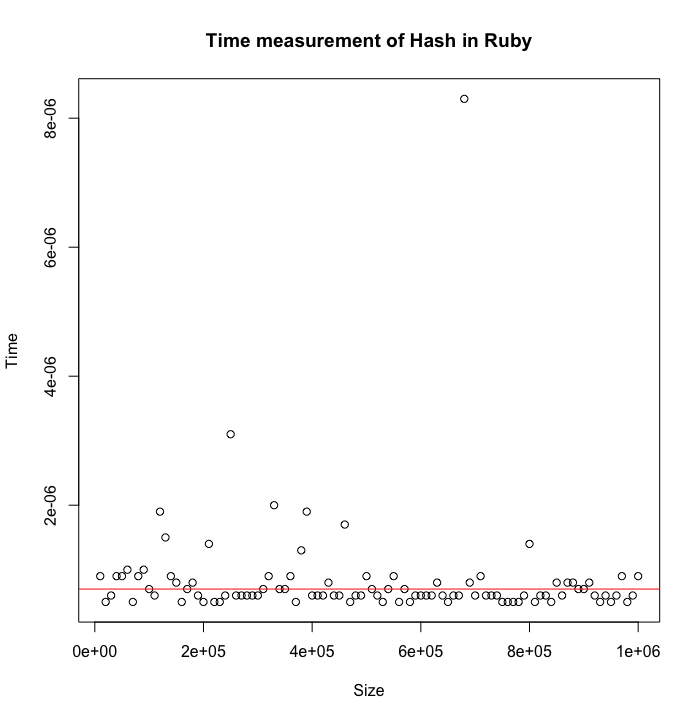
\includegraphics[width=\linewidth]{Rplot2.png}
\end{figure}

\subsubsection{Return of the Spanning Tree}
\subsubsection{Testing the algorithm:}
In this analysis, I test my knapsack function with the size from 10000 to 1000000 and for every case of the size I run 10 times, and then make an average of the time. In addition, I am going to use statistical analysis using the software R.Also, I create a variable called sum which represent the summation of each weight of the item; I create this variable to use in my test as the input of the maximum weight. In the test, I put the maximum weight as the total weight, therefore, I am indirectly sorting the items and testing the same time the worst case scenario. I did the previous implementation to prove that my function runs in O(nlogn).

\paragraph{Fitting the points using linear regression}

$$ TIME = (-1.614e+01) + (2.350e-05)*EDGES $$
$$ p-value: < 2.2e-16 $$
$$ RSE: 13.29 $$
$$ R^{2}:  0.9944 $$
$$ F-statistic: 1.197e+04 $$

\begin{figure}[H]
\centering
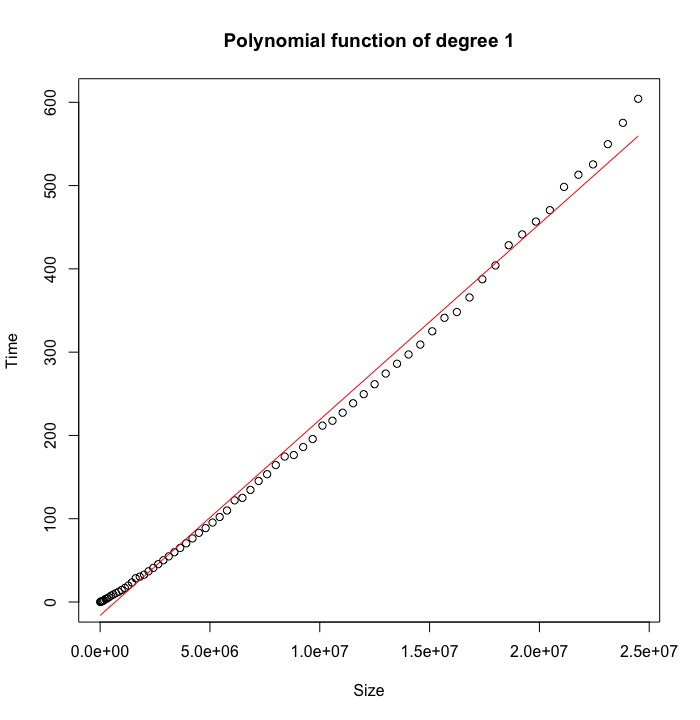
\includegraphics[width=\linewidth]{Rplot3.png}
\caption{Linear Regression}
\end{figure}


\paragraph{Fitting the points using Polynomial regression of grade 2}
$$ TIME = (-1.603) + (1.772e-05)*EDGES +(2.705e-13)*EDGES^{2}$$
$$ p-value: < 2.2e-16 $$
$$ RSE: 3.297  $$
$$ R^{2}:  0.9997 $$
$$ F-statistic:9.787e+04$$

\begin{figure}[H]
\centering
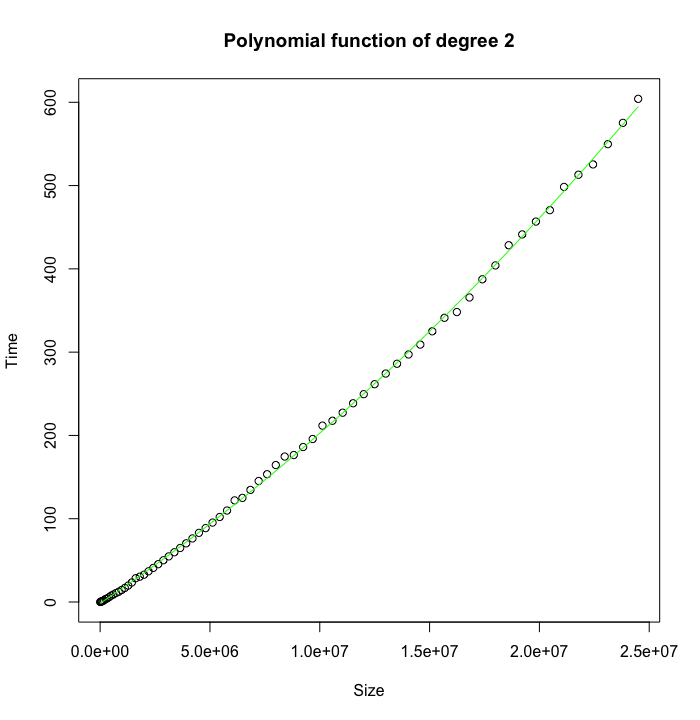
\includegraphics[width=\linewidth]{Rplot4.png}
\caption{Polynomial regression of grade 2}
\end{figure}



\paragraph{Fitting the points using Polynomial regression of grade 3}
$$ TIME = (-2.749) + (1.867e-05)*EDGES  +(1.561e-13)*EDGES^{2} + (3.370e-2)*EDGES^{3}$$
$$ p-value: < 2.2e-16 $$
$$ RSE: 3.162 $$
$$ R^{2}:  0.9997 $$
$$ F-statistic: 7.096e+04$$

\begin{figure}[H]
\centering
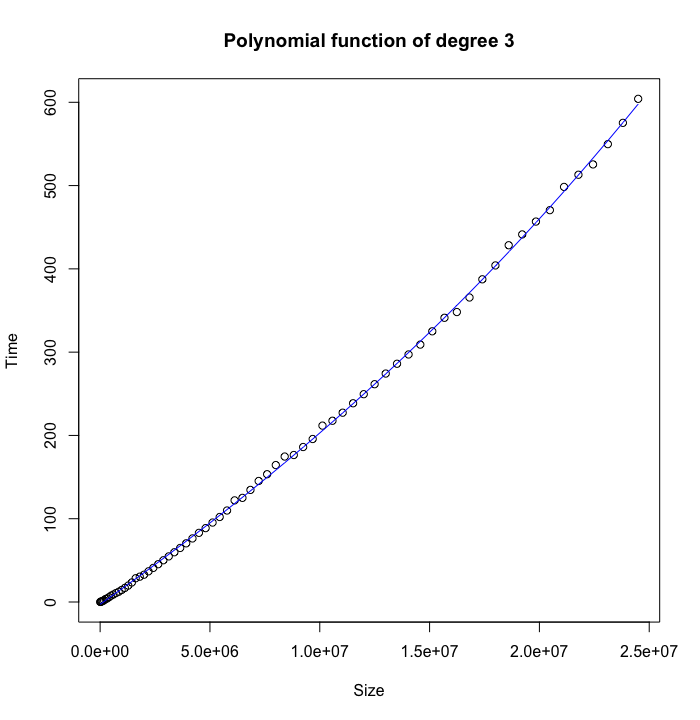
\includegraphics[width=\linewidth]{Rplot5.png}
\caption{Polynomial regression of grade 3}
\end{figure}





\paragraph{Fitting the points using Polynomial regression of grade 4}
$$ TIME = (-1.549e+00) + (1.698e-05)*EDGES  +(5.299e-13)*EDGES^{2} + (-2.267e-20)*EDGES^{3} + (5.613e-28)*EDGES^{4}$$
$$ p-value: < 2.2e-16 $$
$$ RSE: 3.003 $$
$$ R^{2}:  0.9997 $$
$$ F-statistic: 5.9e+04$$

\begin{figure}[H]
\centering
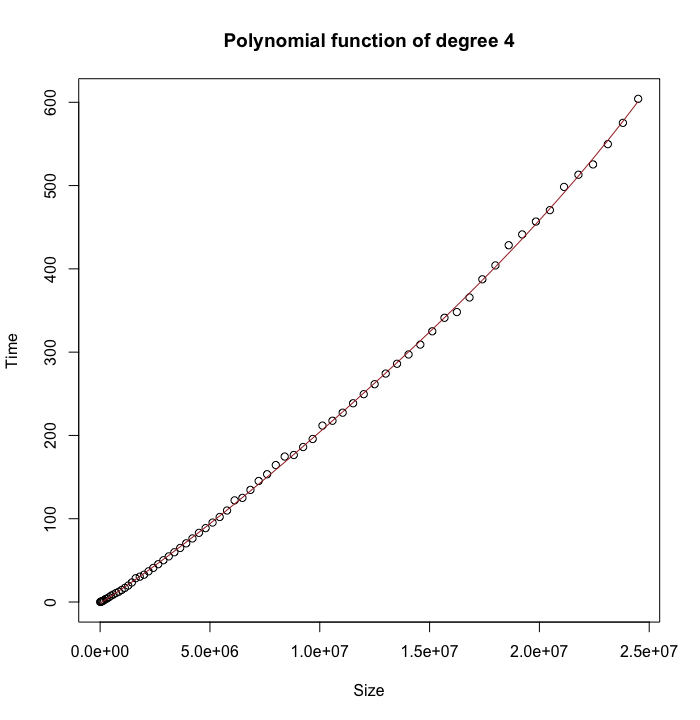
\includegraphics[width=\linewidth]{Rplot6.png}
\caption{Polynomial regression of grade 4}
\end{figure}







\paragraph{Fitting the points using Polynomial regression of grade 5}
$$ TIME = (-2.759e-01) + (1.424e-05)*EDGES  +(1.480e-12)*EDGES^{2} + (-1.372e-19)*EDGES^{3} + (6.158e-27)*EDGES^{4} +
(-9.516e-35)*EDGES^{5}$$
$$ p-value: < 2.2e-16 $$
$$ RSE: 2.808$$
$$ R^{2}:  0.9998 $$
$$ F-statistic: 5.397e+044$$

\begin{figure}[H]
\centering
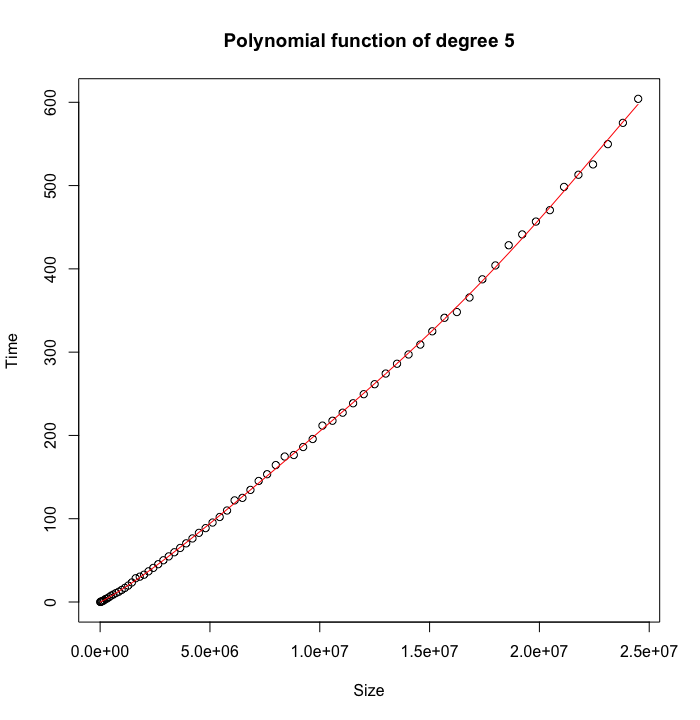
\includegraphics[width=\linewidth]{Rplot7.png}
\caption{Polynomial regression of grade 5}
\end{figure}




\paragraph{Fitting the points using n*log(n) curve}

$$ TIME = (-9.352) + (9.609e-07)*EDGES *log(EDGES)$$
$$ p-value: < 2.2e-16 $$
$$ RSE: 9.608$$
$$ R^{2}:  0.9971$$
$$ F-statistic: 2.299e+04$$

\begin{figure}[H]
\centering
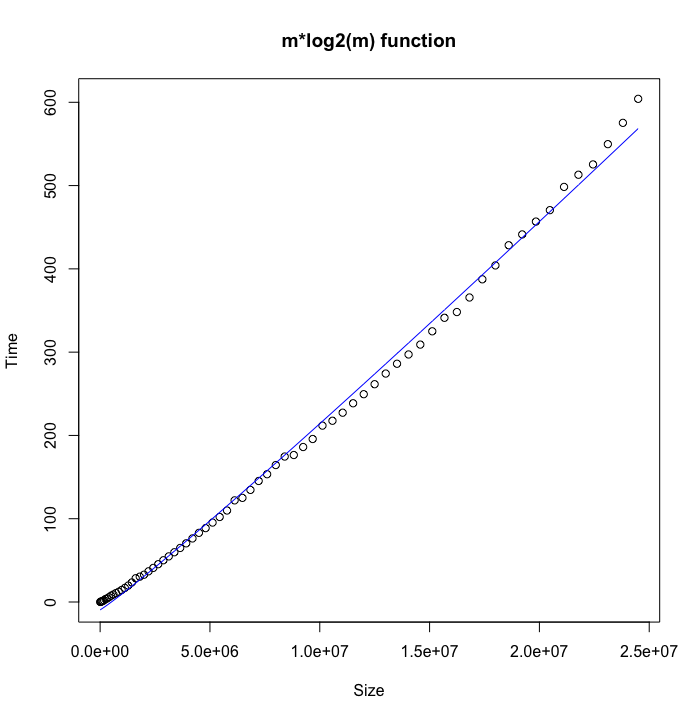
\includegraphics[width=\linewidth]{Rplot8.png}
\caption{nlogn style}
\end{figure}

\paragraph{Fitting the points using n*log(n) curve with addition of functions}

$$ TIME =  (-7.297) + (4.963666e-07)*(EDGES*log(EDGES) + (-1.170e-04)EDGES + (2.319e-02)VERTICES$$
$$ p-value: < 2.2e-16 $$
$$ RSE: 4.308$$
$$ R^{2}:  0.9994$$
$$ F-statistic: 3.82e+04$$

\begin{figure}[H]
\centering
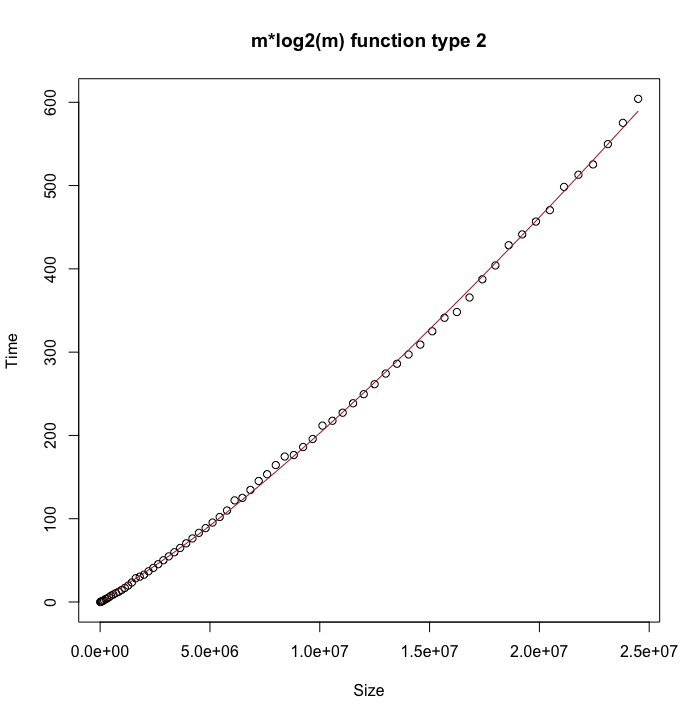
\includegraphics[width=\linewidth]{Rplot9.png}
\caption{nlogn style}
\end{figure}

\subsection{Summary}
In all the cases, the models have presented a $R^{2}$ very near to 1 which tell us that is a good model, also the p-value is less than 0.05 which also tella us that the predictors have influence and is good model, and the F-statistic in all the cases show us that models have high influence. The problem is that the model of polynomial regression on degree 2 show the highest F-statistic which tells us the is the best model to predict. Although that model has the best prediction, it does not neccesary mean that the last model in which there is O(m*log(n)) is incorrect becuase this model present all the statistics varibles with a good value and does not indicate as a bad or inaccurate model.
\\
\lstloadlanguages{R}
\lstset{%
basicstyle=\ttfamily,
commentstyle = \ttfamily\color{black},
keywordstyle=\ttfamily\color{black},
stringstyle=\color{black}}
\lstset{
numbers=left,
numberstyle=\small,
numbersep=8pt,
language=R,
framexleftmargin=2pt}
In addition, I am going to make an analysis to the coefficients with this R code.
\begin{lstlisting}[language=R]
s = (kruskal$time/(kruskal$edges*log2(kruskal$edges)))
summary(s)
    Min.   1st Qu.    Median      Mean   3rd Qu.      Max.
6.129e-07 8.053e-07 8.644e-07 8.458e-07 8.962e-07 1.005e-06
\end{lstlisting}
The mean show us a value of $8.458e-07$ which is very low and represent as the coefficient to multiplicate to obtain the time. The coefficient in the model 2 is $2.705e-13$ which is lower than  $8.458e-07$ which mean that the function need a very small number to maintain the correct prediction and help us to show that this model is not representing a quadratic growth.Also, the coefficient in the last model is $4.963666e-07$ which almost half of the mean and it gives us a hint about how is going to be the growth of the function, therefore coefficient makes sense in our intuition of choosing the correct model.




\end{document}
